\documentclass{beamer}


\usepackage[french,english]{babel}

\usepackage[T1]{fontenc}

\usepackage[utf8]{inputenc}
\usepackage[linesnumbered,ruled,vlined]{algorithm2e}

\usetheme{Warsaw}
\title{Apprentissage et résultats}

\author{Clément Legrand}


\begin{document}
\footnotesize

\begin{frame}[plain]
\titlepage
\end{frame}

\section{Apprentissage}

\subsection{Description}

\begin{frame}{Description}
\begin{block}{Base de départ}
Les solutions données par CW.
\begin{itemize}
\item Tirage au sort de N triplets ($\lambda$, $\mu$, $\nu$);
\item Calcul des solutions pour tout triplet ($\lambda$, $\mu$, $\nu$).
\end{itemize}
\end{block}

\begin{block}{Base d'apprentissage}
On peut ne garder qu'une partie de la base générée pour apprendre
\begin{itemize}
\item On garde $x\%$ des meilleures solutions (quantité privilégiée, Quan$_{x}$);
\item On garde les solutions qui ont un coût inférieur à $c_{min} + (c_{max}-c_{min})\frac{x}{100}$ (qualité privilégiée, Qual$_{x}$).
\item On choisit d'utiliser toute la base générée pour apprendre (Tout)
\end{itemize}
\end{block}
\end{frame}

\begin{frame}{Protocole}

\begin{exampleblock}{Protocole}
\begin{itemize}
\item Génération d'un échantillon de taille $N_{ech}$
\item Calcul de la base d'apprentissage
\item On initialise une matrice MAT de taille $n^2$
\item Pour chaque arête (a,b) on incrémente la valeur MAT[a][b] (si a>b, on commence par échanger a et b)
\item Comparaison arêtes obtenues et optimales.
\end{itemize}
\end{exampleblock}

\begin{block}{Choix des arêtes}
\begin{itemize}
\item On conserve (a,b) si MAT[a][b] dépasse une certaine valeur (Seuil);
\item On conserve les k premières arêtes en triant selon les valeurs contenues dans MAT (Rang).
\end{itemize}
\end{block}

\end{frame}

\subsection{Résultats A-n37-k06}

\begin{frame}{Instance test}
3 instances ont été choisies pour réaliser ces tests: A-n37-k06, A-n65-k09 et P-n101-k04.

La solution employée pour comparer les résultats est celle de la littérature.

La meilleure solution comporte 42 arêtes.

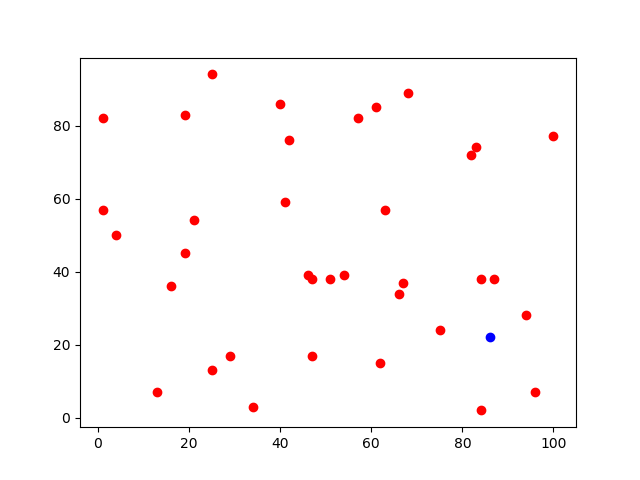
\includegraphics[scale=0.3]{instance3706.png}
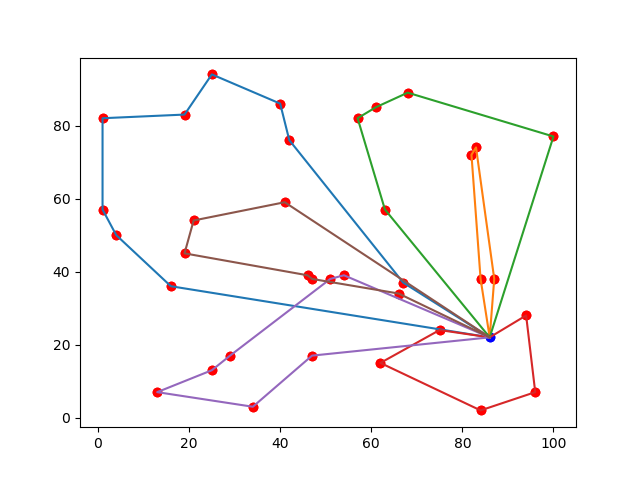
\includegraphics[scale=0.3]{best3706.png}

Pour chaque test on effectue 5 itérations.

Temps de calcul: 2 s (50), 4 s (100), 20 s (500), 44 s (1000).
\end{frame}

\begin{frame}{Résultats A-n37-k06, critère Seuil}

\begin{table}[H]

\begin{tabular}{|@{}c@{}|@{}c@{}|@{}c@{}|@{}c@{}|@{}c@{}||@{}c@{}|@{}c@{}|@{}c@{}|@{}c@{}||@{}c@{}|@{}c@{}|@{}c@{}|@{}c@{}|}

\hline
 & \multicolumn{4}{c|}{Quan$_{10}$} & \multicolumn{4}{c|}{Qual$_{10}$} & \multicolumn{4}{c|}{Tout} \\
 \hline
 & Seuil & Arêtes & Corr & Prop & Seuil & Arêtes & Corr & Prop & Seuil & Arêtes & Corr & Prop \\
 \hline
 50 & 3 & 34 & 21 & 0.5 & 11 & 33 & 21 & 0.50 & 25 & 23 & 15 & 0.35 \\
 \cline{2-13} 
    & 4 & 23 & 14 & 0.33 & 17 & 17 & 12 & 0.28 & 38 & 10 & 7 & 0.16 \\
  \hline
   100 & 5 & 30 & 21 & 0.5 & 15 & 31 & 23 & 0.55 & 50 & 24 & 17 & 0.40 \\
 \cline{2-13} 
    & 8 & 16 & 15 & 0.36 & 23 & 17 & 14 & 0.33 & 75 & 6 & 6 & 0.14 \\
  \hline
   500 & 25 & 32 & 24 & 0.57 & 58 & 31 & 22 & 0.52 & 250 & 22 & 15 & 0.36 \\
 \cline{2-13} 
    & 38 & 15 & 14 & 0.33 & 88 & 20 & 16 & 0.38 & 375 & 7 & 7 & 0.18 \\
  \hline
   Complet & 400 & 33 & 24 & 0.57 & 732 & 30 & 23 & 0.55 & 4000 & 25 & 16 & 0.38 \\
 \cline{2-13} 
    & 600 & 15 & 14 & 0.33 & 1097 & 18 & 16 & 0.38 & 6000 & 9 & 6 & 0.14 \\
  \hline

\end{tabular}
\end{table}
\begin{itemize}
\item Taille de l'échantillon ne semble pas avoir d'influence sur les résultats (\emph{prop} reste semblable quel que soit la taille de l'échantillon).
\item Avec base \emph{Tout} : valeurs de \emph{prop} plus basses $\rightarrow$ pas la peine d'utiliser tout l'échantillon.
\end{itemize}

Remarque : Base Quan$_{10}$ trop petite avec échantillon 50 ou 100.


\end{frame}

\begin{frame}{Résultats A-n37-k06, critère Rang}
\begin{table}[H]

\begin{tabular}{|@{}c@{}|@{}c@{}|@{}c@{}|@{}c@{}||@{}c@{}|@{}c@{}|@{}c@{}||@{}c@{}|@{}c@{}|@{}c@{}|}

\hline
 & \multicolumn{3}{c|}{Quan$_{10}$} & \multicolumn{3}{c|}{Qual$_{10}$} & \multicolumn{3}{c|}{Tout} \\
 \hline
 & Rang & Corr & Prop & Rang & Corr & Prop & Rang & Corr & Prop \\
 \hline
 50 & 10  & 6 & 0.14 & 10  & 6 & 0.14 & 10  & 7 & 0.16  \\
 \cline{2-10} 
    & 20 & 13 & 0.31 & 20  & 13 & 0.32 & 20  & 13 & 0.31  \\
 \cline{2-10} 
    & 18 & 12 & 0.28 & 18 & 13 & 0.3 & 18 & 12 & 0.28  \\
  \hline
   100 & 10  & 9 & 0.21 & 10  & 9 & 0.21 & 10  & 10 & 0.24  \\
 \cline{2-10} 
    & 20 & 16 & 0.38 & 20 & 16 & 0.38 & 20 & 15 & 0.36  \\
  \cline{2-10} 
    & 18 & 13 & 0.3 & 18 & 13 & 0.3 & 18 & 12 & 0.29  \\
  \hline
   500 & 10  & 9 & 0.21 & 10  & 10 & 0.24 & 10  & 9 & 0.21  \\
 \cline{2-10} 
    & 20 & 16 & 0.38 & 20 & 16 & 0.38 & 20 & 15 & 0.36  \\
  \cline{2-10} 
    & 18 & 13 & 0.3 & 18 & 13 & 0.3 & 18 & 12 & 0.28  \\
  \hline
   Complet & 10 & 8 & 0.19 & 10 & 9 & 0.21 & 10 & 7 & 0.17  \\
 \cline{2-10} 
    & 20 & 14 & 0.33 & 20 & 14 & 0.33 & 20 & 14 & 0.33  \\
  \cline{2-10} 
    & 18 & 12 & 0.29 & 18 & 12 & 0.29 & 18 & 12 & 0.29  \\
  \hline

\end{tabular}
\end{table}

Les 3 bases fournissent des valeurs \emph{prop} similaires.
\end{frame}
\subsection{Résultats A-n65-k09}

\begin{frame}{Instance test}

La solution employée pour comparer les résultats est celle de la littérature.

La meilleure solution comporte 73 arêtes.

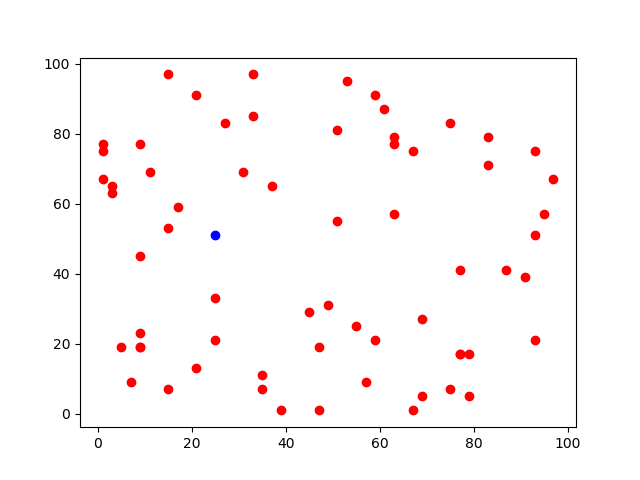
\includegraphics[scale=0.3]{Instance6509.png}
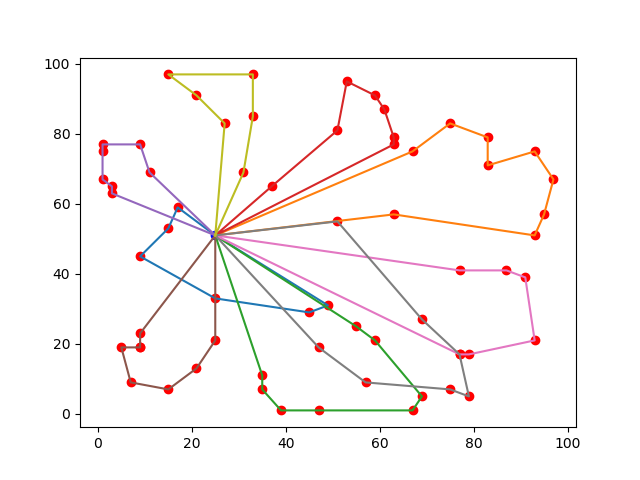
\includegraphics[scale=0.3]{Solution6509.png}

Pour chaque test on effectue 5 itérations.

Temps de calcul: 4 s (50), 8 s (100), 42 s (500), 84 s (1000).
\end{frame}

\begin{frame}{Résultats A-n65-k09, critère Seuil}

\begin{table}[H]

\begin{tabular}{|@{}c@{}|@{}c@{}|@{}c@{}|@{}c@{}|@{}c@{}||@{}c@{}|@{}c@{}|@{}c@{}|@{}c@{}||@{}c@{}|@{}c@{}|@{}c@{}|@{}c@{}|}

\hline
 & \multicolumn{4}{c|}{Quan$_{10}$} & \multicolumn{4}{c|}{Qual$_{10}$} & \multicolumn{4}{c|}{Tout} \\
 \hline
 & Seuil & Arêtes & Corr & Prop & Seuil & Arêtes & Corr & Prop & Seuil & Arêtes & Corr & Prop \\
 \hline
 50 & 3 & 73 & 43 & 0.59 & 10 & 64 & 44 & 0.60 & 25 & 40 & 31 & 0.43 \\
 \cline{2-13} 
    & 4 & 61 & 40 & 0.55 & 15 & 39 & 29 & 0.40 & 38 & 14 & 9 & 0.13 \\
  \hline
   100 & 5 & 70 & 44 & 0.6 & 22 & 58 & 42 & 0.58 & 50 & 43 & 33 & 0.45 \\
 \cline{2-13} 
    & 8 & 63 & 41 & 0.56 & 33 & 36 & 28 & 0.39 & 75 & 15 & 10 & 0.14 \\
  \hline
   500 & 25 & 71 & 43 & 0.59 & 111 & 56 & 41 & 0.56 & 250 & 45 & 35 & 0.48 \\
 \cline{2-13} 
    & 38 & 60 & 40 & 0.55 & 167 & 35 & 28 & 0.39 & 375 & 14 & 9 & 0.13 \\
  \hline
   Complet & 400 & 62 & 41 & 0.56 & 1005 & 56 & 40 & 0.55 & 4000 & 45 & 35 & 0.48 \\
 \cline{2-13} 
    & 600 & 15 & 14 & 0.33 & 1508 & 35 & 28 & 0.39 & 6000 & 13 & 9 & 0.12 \\
  \hline

\end{tabular}


\end{table}

Si trop d'arêtes renvoyées $\rightarrow$ Solutions infaisables ? (futurs tests)


\end{frame}

\begin{frame}{Résultats A-n65-k09, critère Rang}
\begin{table}[H]

\begin{tabular}{|@{}c@{}|@{}c@{}|@{}c@{}|@{}c@{}||@{}c@{}|@{}c@{}|@{}c@{}||@{}c@{}|@{}c@{}|@{}c@{}|}

\hline
 & \multicolumn{3}{c|}{Quan$_{10}$} & \multicolumn{3}{c|}{Qual$_{10}$} & \multicolumn{3}{c|}{Tout} \\
 \hline
 & Rang & Corr & Prop & Rang & Corr & Prop & Rang & Corr & Prop \\
 \hline
 50 & 10  & 6 & 0.08 & 10  & 7 & 0.1 & 10  & 7 & 0.1  \\
 \cline{2-10} 
    & 20 & 14 & 0.2 & 20  & 15 & 0.21 & 20  & 14 & 0.19  \\
 \cline{2-10} 
    & 33 & 23 & 0.32 & 33 & 26 & 0.36 & 33 & 24 & 0.33  \\
  \hline
   100 & 10  & 6 & 0.08 & 10  & 7 & 0.1 & 10  & 7 & 0.1  \\
 \cline{2-10} 
    & 20 & 16 & 0.22 & 20 & 16 & 0.22 & 20 & 14 & 0.19  \\
  \cline{2-10} 
    & 33 & 26 & 0.36 & 33 & 26 & 0.36 & 33 & 25 & 0.34  \\
  \hline
   500 & 10  & 7 & 0.1 & 10  & 7 & 0.1 & 10  & 6 & 0.08  \\
 \cline{2-10} 
    & 20 & 17 & 0.23 & 20 & 15 & 0.21 & 20 & 13 & 0.18  \\
  \cline{2-10} 
    & 33 & 27 & 0.37 & 33 & 26 & 0.36 & 33 & 25 & 0.34  \\
  \hline
   Complet & 10 & 7 & 0.1 & 10 & 7 & 0.1 & 10 & 6 & 0.08  \\
 \cline{2-10} 
    & 20 & 17 & 0.23 & 20 & 17 & 0.23 & 20 & 13 & 0.18  \\
  \cline{2-10} 
    & 33 & 27 & 0.37 & 33 & 27 & 0.37 & 33 & 25 & 0.34  \\
  \hline

\end{tabular}
\end{table}

De nouveau les 3 bases renvoient des résultats similaires. 
\end{frame}



\subsection{Résultats P-n101-k04}

\begin{frame}{Instance test}

La solution employée pour comparer les résultats est celle de la littérature.

La meilleure solution comporte 104 arêtes.

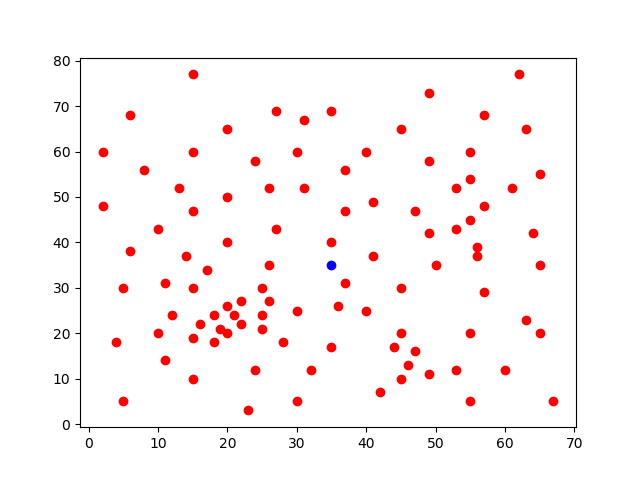
\includegraphics[scale=0.3]{Instance10104.png}
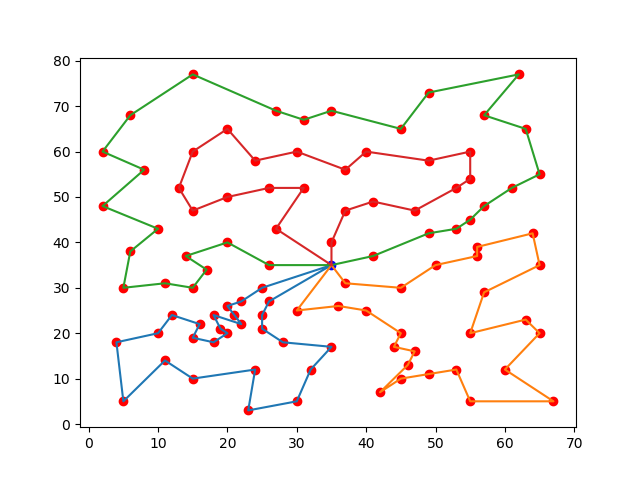
\includegraphics[scale=0.3]{Solution10104.png}

Pour chaque test on effectue 5 itérations.

Temps de calcul: 38 s (50), 75 s (100), 375 s (500), 1060 s (8000). 
\end{frame}
\begin{frame}{Résultats P-n101-k04, critère Seuil}

\begin{table}[H]
\begin{tabular}{|@{}c@{}|@{}c@{}|@{}c@{}|@{}c@{}|@{}c@{}||@{}c@{}|@{}c@{}|@{}c@{}|@{}c@{}||@{}c@{}|@{}c@{}|@{}c@{}|@{}c@{}|}

\hline
 & \multicolumn{4}{c|}{Quan$_{10}$} & \multicolumn{4}{c|}{Qual$_{10}$} & \multicolumn{4}{c|}{Tout} \\
 \hline
 & Seuil & Arêtes & Corr & Prop & Seuil & Arêtes & Corr & Prop & Seuil & Arêtes & Corr & Prop \\
 \hline
 50 & 3 & 93 & 65 & 0.62 & 5 & 83 & 66 & 0.64 & 25 & 71 & 61 & 0.59 \\
 \cline{2-13} 
    & 4 & 54 & 44 & 0.42 & 8 & 42 & 37 & 0.36 & 38 & 24 & 21 & 0.20  \\
  \hline
   100 & 5 & 80 & 66 & 0.64 & 9 & 79 & 66 & 0.63 & 50 & 72 & 62 & 0.60 \\
 \cline{2-13} 
    & 8 & 45 & 41 & 0.40 & 14 & 42 & 39 & 0.38 & 75 & 24 & 22 & 0.21 \\
  \hline
   500 & 25 & 83 & 69 & 0.67 & 44 & 81 & 68 & 0.66 & 250 & 72 & 63 & 0.60 \\
 \cline{2-13} 
    & 38 & 43 & 39 & 0.38 & 67 & 39 & 36 & 0.35 & 375 & 22 & 20 & 0.19 \\
  \hline
   Complet & 400 & 87 & 73 & 0.7 & 411 & 85 & 71 & 0.68 & 4000 & 70 & 60 & 0.58 \\
 \cline{2-13} 
    & 600 & 42 & 39 & 0.38 & 616 & 41 & 38 & 0.37 & 6000 & 23 & 21 & 0.2 \\
  \hline

\end{tabular}


\end{table}

Plus la taille de l'instance augmente, et plus la proportion d'arêtes optimales  renvoyées présentes dans la solution optimale est grande.

\end{frame}

\begin{frame}{Résultats P-n101-k04, critère Rang}
\begin{table}[H]

\begin{tabular}{|@{}c@{}|@{}c@{}|@{}c@{}|@{}c@{}||@{}c@{}|@{}c@{}|@{}c@{}||@{}c@{}|@{}c@{}|@{}c@{}|}

\hline
 & \multicolumn{3}{c|}{Quan$_{10}$} & \multicolumn{3}{c|}{Qual$_{10}$} & \multicolumn{3}{c|}{Tout} \\
 \hline
 & Rang & Corr & Prop & Rang & Corr & Prop & Rang & Corr & Prop \\
 \hline
 50 & 10  & 8 & 0.08 & 10  & 8 & 0.08 & 10  & 8 & 0.08 \\
 \cline{2-10} 
    & 20 & 18 & 0.17 & 20  & 17 & 0.16 & 20 & 18 & 0.17  \\
 \cline{2-10} 
    & 50 & 43 & 0.41 & 50 & 44 & 0.43 & 50 & 44 & 0.43  \\
  \hline
   100 & 10  & 8 & 0.08 & 10  & 8 & 0.08 & 10  & 8 & 0.08  \\
 \cline{2-10} 
    & 20 & 18 & 0.17 & 20 & 18 & 0.17 & 20 & 18 & 0.17  \\
  \cline{2-10} 
    & 50 & 46 & 0.44 & 50 & 46 & 0.44 & 50 & 46 & 0.44  \\
  \hline
   500 & 10  & 8 & 0.08 & 10  & 8 & 0.08 & 10  & 8 & 0.08  \\
 \cline{2-10} 
    & 20 & 18 & 0.17 & 20 & 18 & 0.17 & 20 & 18 & 0.17  \\
  \cline{2-10} 
    & 50 & 46 & 0.44 & 50 & 46 & 0.44 & 50 & 46 & 0.44  \\
  \hline
   Complet & 10  & 8 & 0.08 & 10  & 8 & 0.08 & 10  & 8 & 0.08  \\
 \cline{2-10} 
    & 20 & 18 & 0.17 & 20 & 18 & 0.17 & 20 & 18 & 0.17  \\
  \cline{2-10} 
    & 50 & 46 & 0.44 & 50 & 46 & 0.44 & 50 & 46 & 0.44  \\
  \hline

\end{tabular}
\end{table}
Il faut choisir un rang dépendant de la taille de l'instance (rangs fixés à 10 ou 20 ne revoient plus de bons résultats).
\end{frame}

\begin{frame}{Choix de l'échantillon et de la base}
D'après les résultats précédents :
\begin{itemize}
\item Taille échantillon : 50 (aussi efficace que les tailles plus grandes, et plus rapide)
\item Base d'apprentissage : Qual (Quan trop petite pour 50, Tout pas intéressante)
\end{itemize}
Que choisir comme critère pour extraire les arêtes ?
\end{frame}

\begin{frame}{Nouveaux résultats pour les critères}
4 critères : Rang = n/2 ou Rang = n et Seuil = S$_{lb}$/2 ou S$_{lb}$/3
\begin{table}[H]
\begin{tabular}{{|@{}c@{}|@{}c@{}|@{}c@{}|@{}c@{}|@{}c@{}|@{}c@{}|@{}c@{}|@{}c@{}|@{}c@{}|@{}c@{}|@{}c@{}|@{}c@{}|}}

\hline
 \multicolumn{4}{|c|}{A-n37-k06} & \multicolumn{4}{c|}{A-n65-k09} & \multicolumn{4}{c|}{P-n101-k04} \\
 \hline 
 Critère & Arêtes & Corr. & Infais. & Critère & Arêtes & Corr. & Infais. &Critère & Arêtes & Corr. & Infais. \\
 \hline
 Rg = 18 & 18 & 12 & 0 (0) & Rg = 32 & 32 & 25 & 0 (0) & Rg = 50 & 50 & 45 & 0 (0)\\
 \hline
 Rg = 36 & 36 & 22 & 1 (0) & Rg = 64 & 64 & 44 & 2 (1) & Rg = 100 & 100 & 67 & 11 (5)\\
 \hline
 Se = 8 & 45 & 22 & 5 (4) & Se = 9 & 81 & 50 & 17 (11) & Se = 5 & 121 & 56 & 30 (24)\\
 \hline
 Se = 12 & 31 & 20 & 0 (0) & Se = 13 & 59 & 42 & 0 (0) & Se = 8 & 80 & 62 & 2 (1)\\
 \hline
\end{tabular}
\end{table}

\begin{itemize}
\item Critère Rg = n/2 plus précis mais moins d'arêtes
\item Critère Se = S$_{lb}$/2 moins mais plus d'arêtes
\item Les autres critères demandent d'éliminer trop d'arêtes
\end{itemize}

\end{frame}

\section{Intégration de la connaissance dans un algorithme}

\subsection{Présentation algorithme}

\begin{frame}{Algorithme d'optimisation ($H_c$)}

\begin{algorithm}[H]
\DontPrintSemicolon % Some LaTeX compilers require you to use \dontprintsemicolon instead

$Sol \gets CW(\lambda,\mu,\nu)$\;
$NewSol \gets Sol$\;
\While {La dernière amélioration date de moins de 10 sec} {
	Calcul de la pire arête\;
	$NewSol \gets EjectionChain_{FI-RD}$\;
	$NewSol \gets LinKernighan_{BI-O}$\;
	$NewSol \gets CrossExchange_{FI-RD}$\;
	$NewSol \gets LinKernighan_{BI-O}$\;
	\If {$cost(NewSol) < cost(Sol)$} {
		$Sol \gets NewSol$\;
	}

	\If {Pas d'amélioration depuis $n/2$ itérations} {  
		$NewSol \gets Sol$\;
	}
}
\Return{$Sol$}\;

\end{algorithm}

\end{frame}

\begin{frame}{Learning Heuristic}
\begin{algorithm}[H]
\DontPrintSemicolon % Some LaTeX compilers require you to use \dontprintsemicolon instead
$(\lambda^*,\mu^*,\nu^*), Init \gets Apprentissage()$\;
$newBase \gets []$\;
\For {$i \gets 1$ \textbf{to} $10$} {
	\If {$i = 1$} {
		
		\For {$j \gets 1$ \textbf{to} $10$} {
			$Sol \gets H_c(Init,I,D,\lambda^*,\mu^*,\nu^*)$\;
			$newBase \gets newBase \cup Sol$\;
			}	
		
	}
	\Else {
		Déterminer $Init$ avec les connaissances de $newBase$\;
		
		$(\lambda^*,\mu^*,\nu^*), Init \gets Apprentissage(Init)$\;
		
		
		\For {$j \gets 1$ \textbf{to} $10$} {
		 	$Sol \gets H_c(Init,I,D,\lambda^*,\mu^*,\nu^*)$\;
			$newBase \gets newBase \cup Sol$\;
		}
	
	}
}
\Return{La meilleure solution}\;
\end{algorithm}
\end{frame}

\subsection{Résultats}

\begin{frame}{Résultats}

Résultats pour les coûts obtenus
\begin{tabular}{|c|c|c|c|}
   \hline
    & A3706 & A6509 & P10104\\
   \hline
   Best & 952 & 1182 & 692 \\
   \hline
   n/2 & 950 - 954 & 1187 - 1202 & 697 - 714  \\
   \hline
   S$_{lb}$/2 & 957 - 968 & 1205 - 1232 & 697 - 718 \\
   \hline
\end{tabular}

Résultats pour le temps d'exécution (en sec)
\begin{tabular}{|c|c|c|c|}
   \hline
  Instance & A-n37-k06 & A-n65-k09 & P-n101-k04  \\
   \hline
   Temps (app - total) & 8 - 707  & 25 - 814 & 98 - 1110  \\
   \hline
\end{tabular}

problème : temps limite de 10 sec, trop court pour de grandes instances 
\end{frame}

\begin{frame}{Nouveau meilleur résultat}
Pour l'instance Golden-01, nouvelle solution trouvée:


\centering
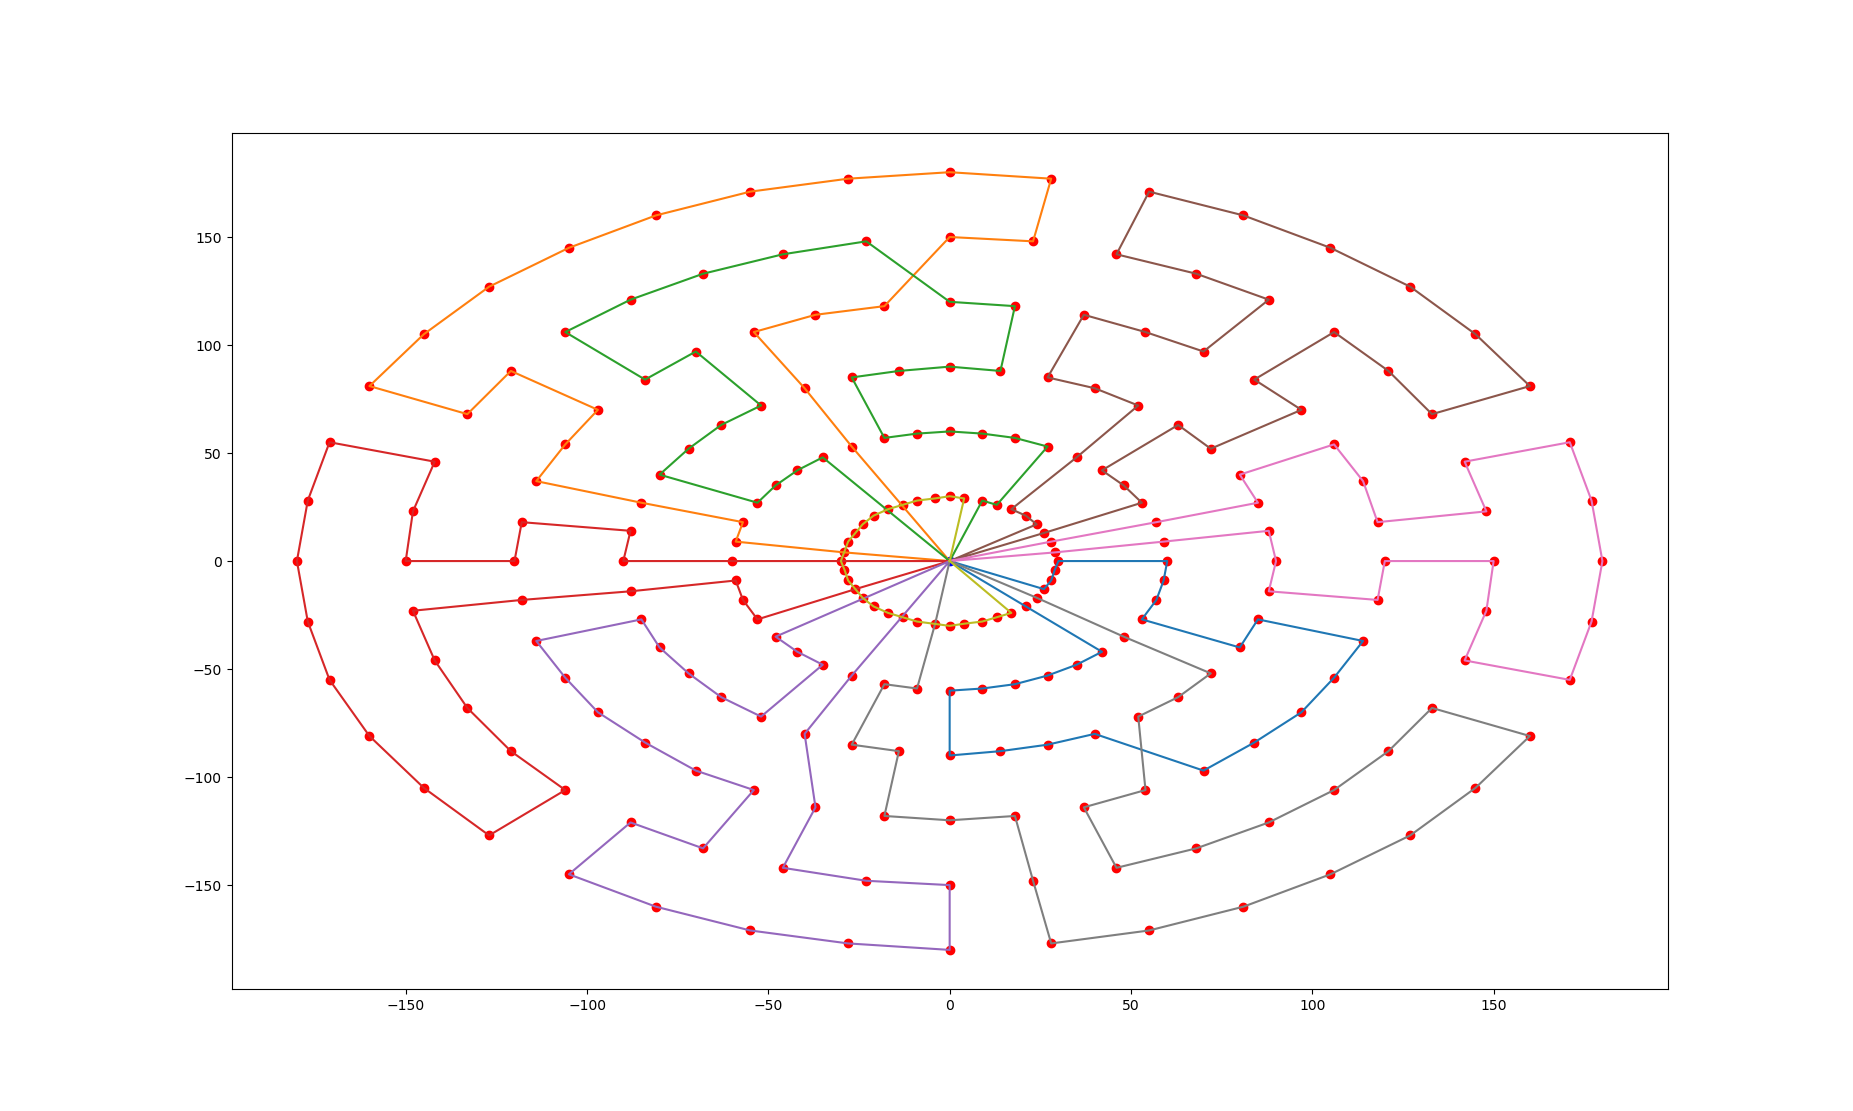
\includegraphics[scale=0.22]{NewREALbest}


Coût de 5563 au lieu de 5623
\end{frame}

\end{document}
